\paragraph{QuizziPedia::Front-End::Directives::MenuBarDirective}

\label{QuizziPedia::Front-End::Directives::MenuBarDirective}

\begin{figure}[h]
	\centering
	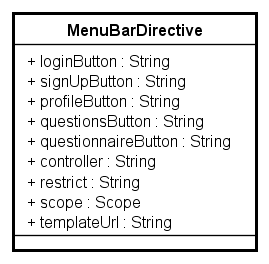
\includegraphics[scale=0.5,keepaspectratio]{UML/Classi/Front-End/QuizziPedia_Front-end_Directives_MenuBarDirective.png}
	\caption{QuizziPedia::Front-End::Directives::MenuBarDirective}
\end{figure}

\begin{itemize}
	\item \textbf{Descrizione}: rappresenta il menù, presente in ogni pagina dell'applicazione, generato in base agli oggetti passati nello \$scope isolato. Fornisce un pulsante per ogni oggetto ricevuto come parametro, ogni pulsante viene rappresentato con un’icona e con un testo. Al click di un pulsante viene invocata la funzione ad esso associata;
	\item \textbf{Utilizzo}: viene utilizzato per realizzare il menù, presente in ogni pagina dell'applicazione, che permette all'utente di selezionare un'opzione in base al contesto in cui si trova:
		\begin{itemize}
			\item Login;
			\item Registrazione;
			\item Ricerca;
			\item Visualizzare il proprio profilo utente;
			\item Gestire le domande create;
			\item Gestire i questionari creati.
		\end{itemize}
	\item \textbf{Relazioni con altre classi}: 
	\begin{itemize}
		\item \textit{IN} \texttt{Index}: 
		\item \textit{IN} \texttt{SearchDirective}: 
		\item \textit{IN} \texttt{LogoutController}: 
		\item \textit{IN} \texttt{MenuBarController}: 
	\end{itemize}
	\item \textbf{Attributi}: 
	\begin{itemize}
		\item ;
	\end{itemize}
	\item \textbf{Metodi}: 
	\begin{itemize}
		\item ;
	\end{itemize}
\end{itemize}

\paragraph{QuizziPedia::Front-End::Directives::NewQuestionButtonDirective}

\label{QuizziPedia::Front-End::Directives::NewQuestionButtonDirective}

\begin{figure}[h]
	\centering
	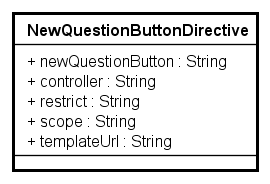
\includegraphics[scale=0.5,keepaspectratio]{UML/Classi/Front-End/QuizziPedia_Front-end_Directives_NewQuestionButtonDirective.png}
	\caption{QuizziPedia::Front-End::Directives::NewQuestionButtonDirective}
\end{figure}

\begin{itemize}
	\item \textbf{Descrizione}: rappresenta il componente grafico che permette all'utente di posizionarsi nella view di creazione di una nuova domanda;
	\item \textbf{Utilizzo}: viene utilizzato per permette all'utente di posizionarsi nella view di creazione di una nuova domanda;
	\item \textbf{Relazioni con altre classi}: 
	\begin{itemize}
		\item \textit{IN} \texttt{QuestionsManagementView}: 
		\item \textit{IN} \texttt{NewQuestionButtonsController}: 
	\end{itemize}
	\item \textbf{Attributi}: 
	\begin{itemize}
		\item ;
	\end{itemize}
	\item \textbf{Metodi}: 
	\begin{itemize}
		\item ;
	\end{itemize}
\end{itemize}

\paragraph{QuizziPedia::Front-End::Directives::OneQuestionDirective}

\label{QuizziPedia::Front-End::Directives::OneQuestionDirective}

\begin{figure}[h]
	\centering
	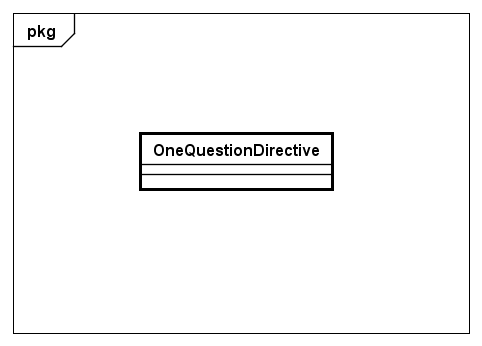
\includegraphics[scale=0.5,keepaspectratio]{UML/Classi/Front-End/QuizziPedia_Front-end_Directives_OneQuestionDirective.png}
	\caption{QuizziPedia::Front-End::Directives::OneQuestionDirective}
\end{figure}

\begin{itemize}
	\item \textbf{Descrizione}: rappresenta il componente grafico che visualizza all'utente l'anteprima della domanda che ha creato. Eseguendo l'azione di click su di essa sarà possibile modificare tale domanda. All'interno di QuestionsManagementsView verranno stampati a video tanti componenti quanti presenti nello scope isolato ad esso associato;
	\item \textbf{Utilizzo}: viene utilizzato per permettere all'utente di visualizzare le domande che ha creato;
	\item \textbf{Relazioni con altre classi}: 
	\begin{itemize}
		\item \textit{IN} \texttt{QuestionsManagementView}: 
	\end{itemize}
	\item \textbf{Attributi}: 
	\begin{itemize}
		\item ;
	\end{itemize}
	\item \textbf{Metodi}: 
	\begin{itemize}
		\item ;
	\end{itemize}
\end{itemize}

\paragraph{QuizziPedia::Front-End::Directives::QuestionTextDirective}

\label{QuizziPedia::Front-End::Directives::QuestionTextDirective}

\begin{figure}[h]
	\centering
	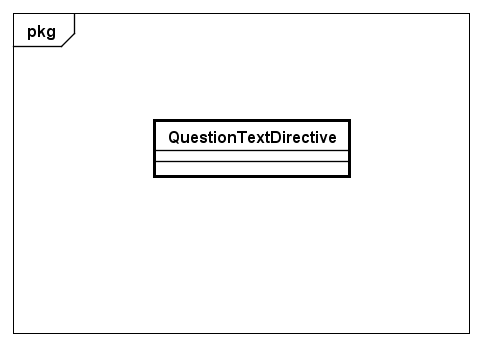
\includegraphics[scale=0.5,keepaspectratio]{UML/Classi/Front-End/QuizziPedia_Front-end_Directives_QuestionTextDirective.png}
	\caption{QuizziPedia::Front-End::Directives::QuestionTextDirective}
\end{figure}

\begin{itemize}
	\item \textbf{Descrizione}: rappresenta il componente grafico che permette all'utente di scrivere o modificare il testo di una domanda;
	\item \textbf{Utilizzo}: viene usato per permettere all'utente di scrivere o modificare il testo di una domanda;
	\item \textbf{Relazioni con altre classi}: 
	\begin{itemize}
		\item \textit{IN} \texttt{TrueFalseQuestionsView}: 
		\item \textit{IN} \texttt{MultipleQuestionsView}: 
		\item \textit{IN} \texttt{ConnectionQuestionsView}: 
		\item \textit{IN} \texttt{ImagesSortingQuestionsView}: 
		\item \textit{IN} \texttt{StringsSortingQuestionsView}: 
		\item \textit{IN} \texttt{FillingQuestionsView}: 
		\item \textit{IN} \texttt{ClickableAreaQuestionsView}: 
	\end{itemize}
	\item \textbf{Attributi}: 
	\begin{itemize}
		\item ;
	\end{itemize}
	\item \textbf{Metodi}: 
	\begin{itemize}
		\item ;
	\end{itemize}
\end{itemize}

\paragraph{QuizziPedia::Front-End::Directives::QuestionnaireDetailsDirective}

\label{QuizziPedia::Front-End::Directives::QuestionnaireDetailsDirective}

\begin{figure}[h]
	\centering
	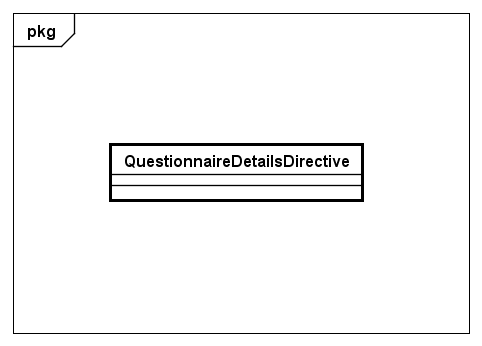
\includegraphics[scale=0.5,keepaspectratio]{UML/Classi/Front-End/QuizziPedia_Front-end_Directives_QuestionnaireDetailsDirective.png}
	\caption{QuizziPedia::Front-End::Directives::QuestionnaireDetailsDirective}
\end{figure}

\begin{itemize}
	\item \textbf{Descrizione}: rappresenta il componente grafico che permette all'utente di visualizzare la lista di questionari che può compilare. Ogni item di questa lista contiene:
		\begin{itemize}
			\item Nome del questionario;
			\item Autore del questionario;
			\item Argomento del questionario;
			\item Parole chiave del questionario;
		\end{itemize}
	Al verificarsi dell'evento click su un item della lista l'utente verrà indirizzato alla view per la compilazione del questionario selezionato;
	\item \textbf{Utilizzo}: viene utilizzato per permettere all'utente di visualizzare la lista di questionari che può compilare;
	\item \textbf{Relazioni con altre classi}: 
	\begin{itemize}
		\item \textit{IN} \texttt{UserView}: 
		\item \textit{IN} \texttt{QuestionnaireDetailsController}: 
	\end{itemize}
	\item \textbf{Attributi}: 
	\begin{itemize}
		\item ;
	\end{itemize}
	\item \textbf{Metodi}: 
	\begin{itemize}
		\item ;
	\end{itemize}
\end{itemize}

\paragraph{QuizziPedia::Front-End::Directives::QuestionnaireDoneDetailsDirective}

\label{QuizziPedia::Front-End::Directives::QuestionnaireDoneDetailsDirective}

\begin{figure}[h]
	\centering
	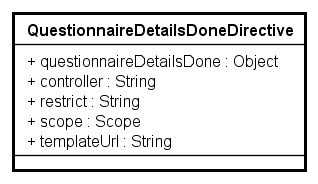
\includegraphics[scale=0.5,keepaspectratio]{UML/Classi/Front-End/QuizziPedia_Front-end_Directives_QuestionnaireDetailsDoneDirective.png}
	\caption{QuizziPedia::Front-End::Directives::QuestionnaireDetailsDoneDirective}
\end{figure}

\begin{itemize}
	\item \textbf{Descrizione}: rappresenta il componente grafico che permette all'utente di visualizzare la lista di questionari che ha già compilato e di conseguenza vederne le valutazioni. Ogni item di questa lista contiene:
	\begin{itemize}
		\item Nome del questionario;
		\item Autore del questionario;
		\item Argomento del questionario;
		\item Parole chiave del questionario;
		\item Valutazione del questionario.
	\end{itemize};
	\item \textbf{Utilizzo}: viene utilizzato per permettere all'utente di visualizzare la lista di questionari che ha compilato;
	\item \textbf{Relazioni con altre classi}: 
	\begin{itemize}
		\item \textit{IN} \texttt{UserView}: 
		\item \textit{IN} \texttt{QuestionnaireDetailsController}: 
	\end{itemize}
	\item \textbf{Attributi}: 
	\begin{itemize}
		\item ;
	\end{itemize}
	\item \textbf{Metodi}: 
	\begin{itemize}
		\item ;
	\end{itemize}
\end{itemize}

\paragraph{QuizziPedia::Front-End::Directives::QuestionsManagementQuestionnaireDirective}

\label{QuizziPedia::Front-End::Directives::QuestionsManagementQuestionnaireDirective}

\begin{figure}[h]
	\centering
	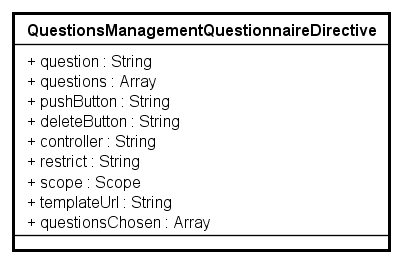
\includegraphics[scale=0.5,keepaspectratio]{UML/Classi/Front-End/QuizziPedia_Front-end_Directives_QuestionsManagementQuestionnaireDirective.png}
	\caption{QuizziPedia::Front-End::Directives::QuestionsManagementQuestionnaireDirective}
\end{figure}

\begin{itemize}
	\item \textbf{Descrizione}: rappresenta il componente grafico che permette all'utente di:
		\begin{itemize}
			\item Effettuare delle ricerche sul database di domande;
			\item Selezionare le domande da inserire nel questionario;
			\item Mostrare le domande già inserite e permettere all'utente di eliminarle da tale lista.
		\end{itemize}
		Questo componente si presta sia per la creazione che per la modifica di un questionario;
	\item \textbf{Utilizzo}: viene utilizzato per gestire le domande di un questionario. Esso permette di ricercare, inserire e togliere domande dalla lista di domande che andranno a comporre il questionario;
	\item \textbf{Relazioni con altre classi}: 
	\begin{itemize}
		\item \textit{IN} \texttt{CreateQuestionnaireView}: 
		\item \textit{IN} \texttt{QuestionnaireQuestionsManagementController}: 
	\end{itemize}
	\item \textbf{Attributi}: 
	\begin{itemize}
		\item ;
	\end{itemize}
	\item \textbf{Metodi}: 
	\begin{itemize}
		\item ;
	\end{itemize}
\end{itemize}